% Provenance (never printed): old terminale S material on absolute dating (the
% decay law recalled, the closed system, the rubidium-strontium isochron) and on
% the history of the age of the Earth (cooling, salt, sediments, then radioactivity,
% meteorites and 4.55 billion years). Owner (Sync 0/1): closed system, isochron,
% age of the Earth (as a defined notion). The decay law, the half-life and the
% dating equation are the physics books' (recalled); relative dating, absolute
% age, superposition, cross-cutting relationships and the eras are Book 1 g7's
% (recalled); the oldest zircons and the Acasta gneiss are g12.01's (quoted).
% Varden Hills granite 310 Ma and schist 480 Ma from figdata/shared/region.py;
% their isotope ratios are exercise data (figdata/grade-12/isochrons.py).
\chapter{Radiometric Dating and the Age of the Earth}\label{ch:g12:age-of-the-earth}

In 1862 the physicist William Thomson, later Lord Kelvin, worked out how old the
Earth is from the way it cools. He supposed that it had formed molten and had
been losing its heat ever since, and asked how long it would take for the
temperature gradient near the surface to fall to its present value. His
answer was 96 million years, somewhere between 20 and 400
million; by 1897 he had narrowed it to between 20 and 40 million.
Geologists found this far too short for the history they read in the rocks.
The answer came from radioactivity, which Kelvin did not know.
% ledger: holmes13:estimates, england:kelvin (Book 3 row)

\begin{omfigure}
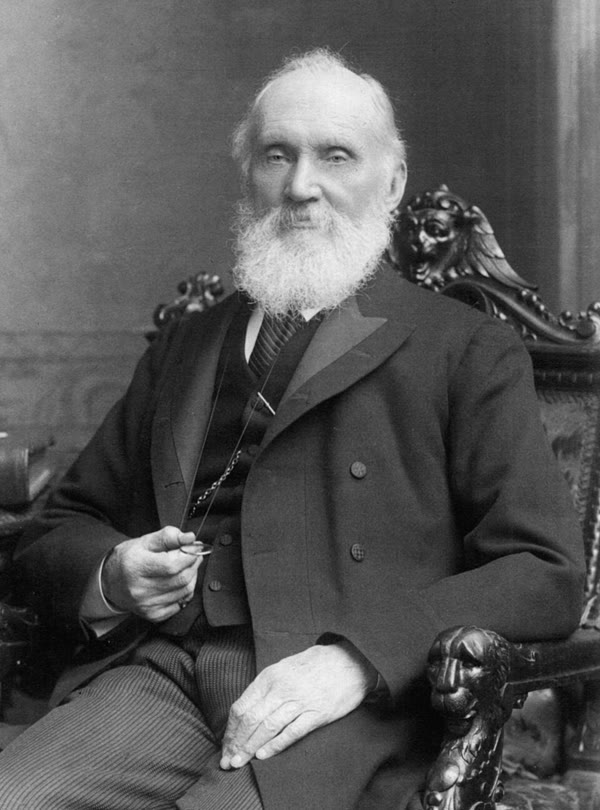
\includegraphics[height=5.2cm]{images/book2/g12-kelvin-1906.jpg}

{\small William Thomson, Lord Kelvin, in 1906. Photograph Russell and Sons,
London (Smithsonian Institution Libraries, no known copyright restrictions).}
\end{omfigure}
% ledger: photo:g12-kelvin

\begin{recall}
Relative dating puts rocks and events in order; an absolute age is a number
of years (Book 1, grade 7). A radioactive isotope, the parent, decays into a
daughter isotope at random: the number $N$ of parent atoms left falls as
$N = N_0\,e^{-\lambda t}$, where $\lambda$ is the decay constant, and halves
every half-life $T = \ln 2/\lambda$ (the physics books). The oldest minerals
known, zircons from Western Australia, are 4.4 billion years old
(\cref{ch:g12:continental-crust}). The Earth also loses heat that radioactivity
keeps making, and its mantle convects (\cref{ch:g12:internal-heat}).
\end{recall}
% ledger: wilde01:zircon

\section{A history of estimates}

Before radioactivity, every estimate of the Earth's age rested on a process
whose rate was supposed known.

\begin{center}
\small
\begin{tabular}{|p{0.19\linewidth}|p{0.42\linewidth}|p{0.25\linewidth}|}
\hline
who, when & method and what it assumes & estimate \\
\hline
Phillips, 1860 & thickness of the sedimentary layers divided by a rate of deposition; assumes a steady rate & 38 to 96 million years \\
Kelvin, 1862 & cooling of a molten Earth by conduction alone, with no source of heat inside & 20 to 400 million years \\
G.\,H.~Darwin & time since the Moon separated from the Earth, from the slowing of their motions by the tides & at least 56 million years \\
Joly, 1899 & salt carried to the sea by rivers, divided by the yearly supply; assumes a steady supply and no salt removed & 80 to 100 million years \\
\hline
\end{tabular}
\end{center}
% ledger: holmes13:estimates

\begin{history}[Kelvin's missing heat]
In 1903 Pierre Curie and Albert Laborde showed that radium gives off heat,
and several scientists soon argued that this heat overturned Kelvin's
conclusion. A year later Ernest Rutherford, lecturing with Kelvin in
the audience, reminded him that he had limited the \omterm{def:g12:age-of-the-earth:age}{age of the Earth}
``provided no new source of heat was discovered''. Radioactivity seemed to be
that source. Yet it was not Kelvin's main error: what most lengthens the Earth's cooling
is \omterm{def:g12:internal-heat:convection}{mantle convection}, which keeps the upper mantle hot and the gradient in
the crust high for far longer than conduction alone would.
\end{history}
% ledger: england:kelvin (Book 3 row)

Radioactivity also gave a clock. In 1907 Bertram Boltwood showed that
uranium minerals of the same age hold the same amount of lead for each gram
of uranium: the lead is made by the uranium. By 1913 Arthur Holmes could
write that the oldest rocks dated were \num{1600} million years old, and in
1927 he put the Earth's age between 1.6 and 3.0 billion years. In 1956 Clair
Patterson measured 4.55 billion years. Today's value is 4.54 billion years,
to within one per cent.
% ledger: holmes13:estimates, holmes27:age, patterson56:table, usgs:age-earth (Book 1 row)

\begin{omfigure}
\begin{tikzpicture}
\begin{axis}[omrecord, width=0.78\linewidth, height=6.2cm, ymode=log, xmin=1840, xmax=2040,
  ymin=1e7, ymax=2e10, xlabel={year of the estimate}, ylabel={estimated age of the Earth (years)},
  xtick={1850,1875,...,2025}, x tick label style={/pgf/number format/.cd, set thousands separator={}},
  ytick={1e7,1e8,1e9,1e10}, ymajorgrids=true, xmajorgrids=false]
% computed in figdata/grade-12/isochrons.py; ledger: holmes13:estimates, holmes27:age, patterson56:table, usgs:age-earth (Book 1 row)
\addplot[omDef, only marks, mark=*, mark size=1.8pt, error bars/.cd, y dir=both, y explicit]
  table[x=year, y=mid, y error minus expr=\thisrow{mid}-\thisrow{lo}, y error plus expr=\thisrow{hi}-\thisrow{mid}]
  {figdata/out/grade-12-isochrons-history.dat};
\addplot[omThm, densely dashed, domain=1840:2040, samples=2] {4.54e9};
\coordinate (k62) at (axis cs:1862,2.4e8);
\coordinate (k97) at (axis cs:1897,2.8e7);
\coordinate (jol) at (axis cs:1899,1e8);
\coordinate (h11) at (axis cs:1919,1.3e9);
\coordinate (pat) at (axis cs:1956,4.55e9);
\coordinate (now) at (axis cs:1845,4.54e9);
\end{axis}
\node[font=\scriptsize, anchor=west] at ([xshift=4pt]k62) {Kelvin 1862};
\node[font=\scriptsize, anchor=east] at ([xshift=-4pt]k97) {Kelvin 1897};
\node[font=\scriptsize, anchor=west] at ([xshift=4pt]jol) {Joly};
\node[font=\scriptsize, anchor=north] at (h11) {Holmes};
\node[font=\scriptsize, anchor=north west] at ([xshift=2pt, yshift=-3pt]pat) {Patterson};
\node[font=\scriptsize, text=omThm, anchor=south west] at (now) {today, 4.54 billion years};
\end{tikzpicture}

{\small Estimates of the \omterm{def:g12:age-of-the-earth:age}{age of the Earth} against the year they were made, on
a logarithmic scale; bars span the range each author gave. Holmes's 1913
point is the age of the oldest rocks then dated, a minimum. Sources: Holmes
(1913, 1927); Patterson (1956); U.S. Geological Survey.}
\end{omfigure}

\section{A radioactive clock}

A radioactive clock works only if nothing has been added to it or taken
away since it started.

\begin{definition}[Closed system]\label{def:g12:age-of-the-earth:closed-system}
A rock or a mineral is a \emph{closed system}\index{closed system} for a
parent isotope and its daughter if, since the moment its clock started,
no atom of the parent or of the daughter has entered or left it, other than
by the decay of the parent into the daughter.
\end{definition}
% ledger: tulane:radiometric

For a mineral the clock starts when it crystallises from a magma, or more
exactly when it has cooled enough for the atoms to stop moving in and out of
it. Heating, a hot
fluid or weathering can open the system again, and the age then measured is
wrong, or dates that later event.
% ledger: tulane:radiometric

Counting the daughter atoms in a \omterm{def:g12:age-of-the-earth:closed-system}{closed system} gives the age, provided one
knows how many were there at the start. Usually one does not. Rubidium-87
decays into strontium-87, but every mineral also took in some strontium-87
when it formed. The \omterm{def:g12:age-of-the-earth:isochron}{isochron} method gets round this by measuring several
minerals of one rock.

\section{The isochron}

Strontium has an isotope, strontium-86, that is stable and made by no
decay: in a \omterm{def:g12:age-of-the-earth:closed-system}{closed system} its number stays the same, and it serves as a
yardstick. The isotope ratios $^{87}\mathrm{Sr}/^{86}\mathrm{Sr}$ and
$^{87}\mathrm{Rb}/^{86}\mathrm{Sr}$ are what a mass spectrometer measures.

\begin{theorem}[The isochron equation]\label{thm:g12:age-of-the-earth:isochron}
In a mineral that has been a \omterm{def:g12:age-of-the-earth:closed-system}{closed system} for a time $t$,
\[
  \left(\frac{^{87}\mathrm{Sr}}{^{86}\mathrm{Sr}}\right)_{\text{now}}
  = \left(\frac{^{87}\mathrm{Sr}}{^{86}\mathrm{Sr}}\right)_{0}
  + \left(\frac{^{87}\mathrm{Rb}}{^{86}\mathrm{Sr}}\right)_{\text{now}}
  \left(e^{\lambda t} - 1\right),
\]
where the index 0 marks the value when the clock started and $\lambda$ is
the decay constant of rubidium-87.
\end{theorem}

\begin{proof}
Let $P$ be the number of rubidium-87 atoms now and $P_0$ when the clock
started. By the decay law $P = P_0\,e^{-\lambda t}$, so $P_0 = P\,e^{\lambda t}$,
and the number of atoms that have decayed is $P_0 - P = P\,(e^{\lambda t}-1)$.
In a \omterm{def:g12:age-of-the-earth:closed-system}{closed system} each of them has become one atom of strontium-87, which
is added to the $D_0$ atoms present at the start: $D = D_0 + P\,(e^{\lambda
t}-1)$. Dividing by the number of strontium-86 atoms, which has not changed,
gives the equation.
\end{proof}
% ledger: tulane:radiometric

The minerals of a granite crystallised from one magma, so they all started
with the same ratio $(^{87}\mathrm{Sr}/^{86}\mathrm{Sr})_0$. But they took in
very different amounts of rubidium. All of them share the same $t$ and the same starting ratio, so the
equation says that their points lie on one straight line.

\begin{definition}[Isochron]\label{def:g12:age-of-the-earth:isochron}
An \emph{isochron}\index{isochron} is the straight line on which lie the
points of minerals or rocks that formed at the same time from the same
source and have stayed \omterm{def:g12:age-of-the-earth:closed-system}{closed systems} since, when the ratio of daughter to
stable isotope is plotted against the ratio of parent to stable isotope. Its
slope gives their age, and the point where it meets the vertical axis gives
their starting ratio.
\end{definition}
% ledger: tulane:radiometric

\begin{proposition}[Age from the slope]\label{prop:g12:age-of-the-earth:slope}
If an \omterm{def:g12:age-of-the-earth:isochron}{isochron} has slope $m$, the age is
\[
  t = \frac{\ln(1+m)}{\lambda}.
\]
\end{proposition}

\begin{proof}
Comparing with the \omterm{def:g12:age-of-the-earth:isochron}{isochron} equation, $m = e^{\lambda t} - 1$, so
$e^{\lambda t} = 1 + m$, $\lambda t = \ln(1+m)$, and $t = \ln(1+m)/\lambda$.
\end{proof}

For rubidium-87, $\lambda = \num{1.3972e-11}$ per year, a half-life of
$\ln 2/\lambda \approx 49.6$ billion years: more than ten times the \omterm{def:g12:age-of-the-earth:age}{age of the
Earth}.
% ledger: villa22:rb87

\begin{method}[Dating a rock with an isochron]\label{met:g12:age-of-the-earth:isochron}
\begin{enumerate}
  \item Separate several minerals of the rock (or take several samples of
        it) with different amounts of rubidium.
  \item Measure in each the ratios $^{87}\mathrm{Rb}/^{86}\mathrm{Sr}$ ($x$)
        and $^{87}\mathrm{Sr}/^{86}\mathrm{Sr}$ ($y$).
  \item Plot $y$ against $x$ and check that the points lie on a straight
        line: if one does not, that sample was not a \omterm{def:g12:age-of-the-earth:closed-system}{closed system}.
  \item Take the slope $m$ of the line, and compute $t = \ln(1+m)/\lambda$.
  \item Read the starting ratio where the line meets the vertical axis.
\end{enumerate}
\end{method}

\begin{example}[The Varden granite]\label{ex:g12:age-of-the-earth:varden}
The granite of the Varden Hills, the series' invented region, gives these
ratios (exercise data):
\begin{center}
\small
\begin{tabular}{|l|c|c|}
\hline
sample & $^{87}\mathrm{Rb}/^{86}\mathrm{Sr}$ & $^{87}\mathrm{Sr}/^{86}\mathrm{Sr}$ \\
\hline
plagioclase & 0.35 & 0.70952 \\
hornblende  & 1.20 & 0.71321 \\
whole rock  & 3.10 & 0.72146 \\
K-feldspar  & 6.40 & 0.73578 \\
biotite     & 24.0 & 0.81218 \\
\hline
\end{tabular}
\end{center}
Through the plagioclase and the biotite, the slope is
$m = (0.81218 - 0.70952)/(24.0 - 0.35) \approx 0.004341$. Then
$t = \ln(1.004341)/\num{1.3972e-11} \approx \num{3.10e8}$ years:
the granite is 310 million years old. The line meets the vertical axis at
$0.70952 - 0.35 \times 0.004341 \approx 0.7080$, the starting ratio.
\end{example}
% values: granite_age_Ma 310.0, granite_intercept 0.70800 (isochrons.py)

\begin{omfigure}
\begin{tikzpicture}
\begin{axis}[omrecord, width=0.7\linewidth, height=6cm, xmin=0, xmax=26, ymin=0.695, ymax=0.82, ytick={0.70,0.72,...,0.82},
  xlabel={$^{87}\mathrm{Rb}/^{86}\mathrm{Sr}$}, ylabel={$^{87}\mathrm{Sr}/^{86}\mathrm{Sr}$},
  y tick label style={/pgf/number format/.cd, fixed, fixed zerofill, precision=2}]
% computed in figdata/grade-12/isochrons.py (exercise data, Varden granite 310 Ma); ledger: villa22:rb87
\addplot[omDef, line width=0.9pt] table[x=x, y=y] {figdata/out/grade-12-isochrons-graniteln.dat};
\addplot[omThm, only marks, mark=*, mark size=2pt] table[x=rbsr, y=srsr] {figdata/out/grade-12-isochrons-granite.dat};
\addplot[black!60, densely dotted, domain=0:26, samples=2] {0.7080};
\coordinate (pl) at (axis cs:0.35,0.70952);
\coordinate (hb) at (axis cs:1.2,0.71321);
\coordinate (wr) at (axis cs:3.1,0.72146);
\coordinate (kf) at (axis cs:6.4,0.73578);
\coordinate (bt) at (axis cs:24,0.81218);
\coordinate (sl) at (axis cs:12,0.762);
\coordinate (in) at (axis cs:9,0.7082);
\coordinate (plhb) at (axis cs:0.6,0.737);
\coordinate (plhbpt) at (axis cs:0.9,0.7125);
\end{axis}
\node[font=\scriptsize, anchor=north west] at ([xshift=1pt]wr) {whole rock};
\node[font=\scriptsize, anchor=north west] at ([xshift=1pt]kf) {K-feldspar};
\node[font=\scriptsize, anchor=east] at ([xshift=-3pt]bt) {biotite};
\node[font=\scriptsize, anchor=south west, align=left, inner sep=1pt] (plhblab) at (plhb) {plagioclase,\\hornblende};
\draw[black!60, line width=0.4pt] (plhblab.south) -- (plhbpt);
\node[font=\scriptsize, text=omDef, anchor=south east] at (sl) {slope $0.004341$: 310 million years};
\node[font=\scriptsize, text=black!70, anchor=south west] at (in) {starting ratio 0.7080 (time 0)};
\end{tikzpicture}

{\small The rubidium--strontium \omterm{def:g12:age-of-the-earth:isochron}{isochron} of the Varden granite (exercise
data). When the granite formed, all its minerals lay on the dotted
horizontal line; since then each has risen in proportion to its rubidium, and
they now lie on the solid line.}
\end{omfigure}

\begin{inthelab}[Weighing atoms]
The ratios are measured with a mass spectrometer. A few milligrams of a
mineral are dissolved in acid, and the strontium is separated from the
rubidium by chemistry, since the two isotopes of mass 87 would otherwise be
counted together. The strontium, deposited on a metal filament and heated
in a vacuum, gives off ions; an electric field speeds them up and a magnet
bends their paths, the lighter ions more than the heavier ones, so that each
isotope reaches its own collector. Their currents give the ratios.
\end{inthelab}

\begin{omfigure}
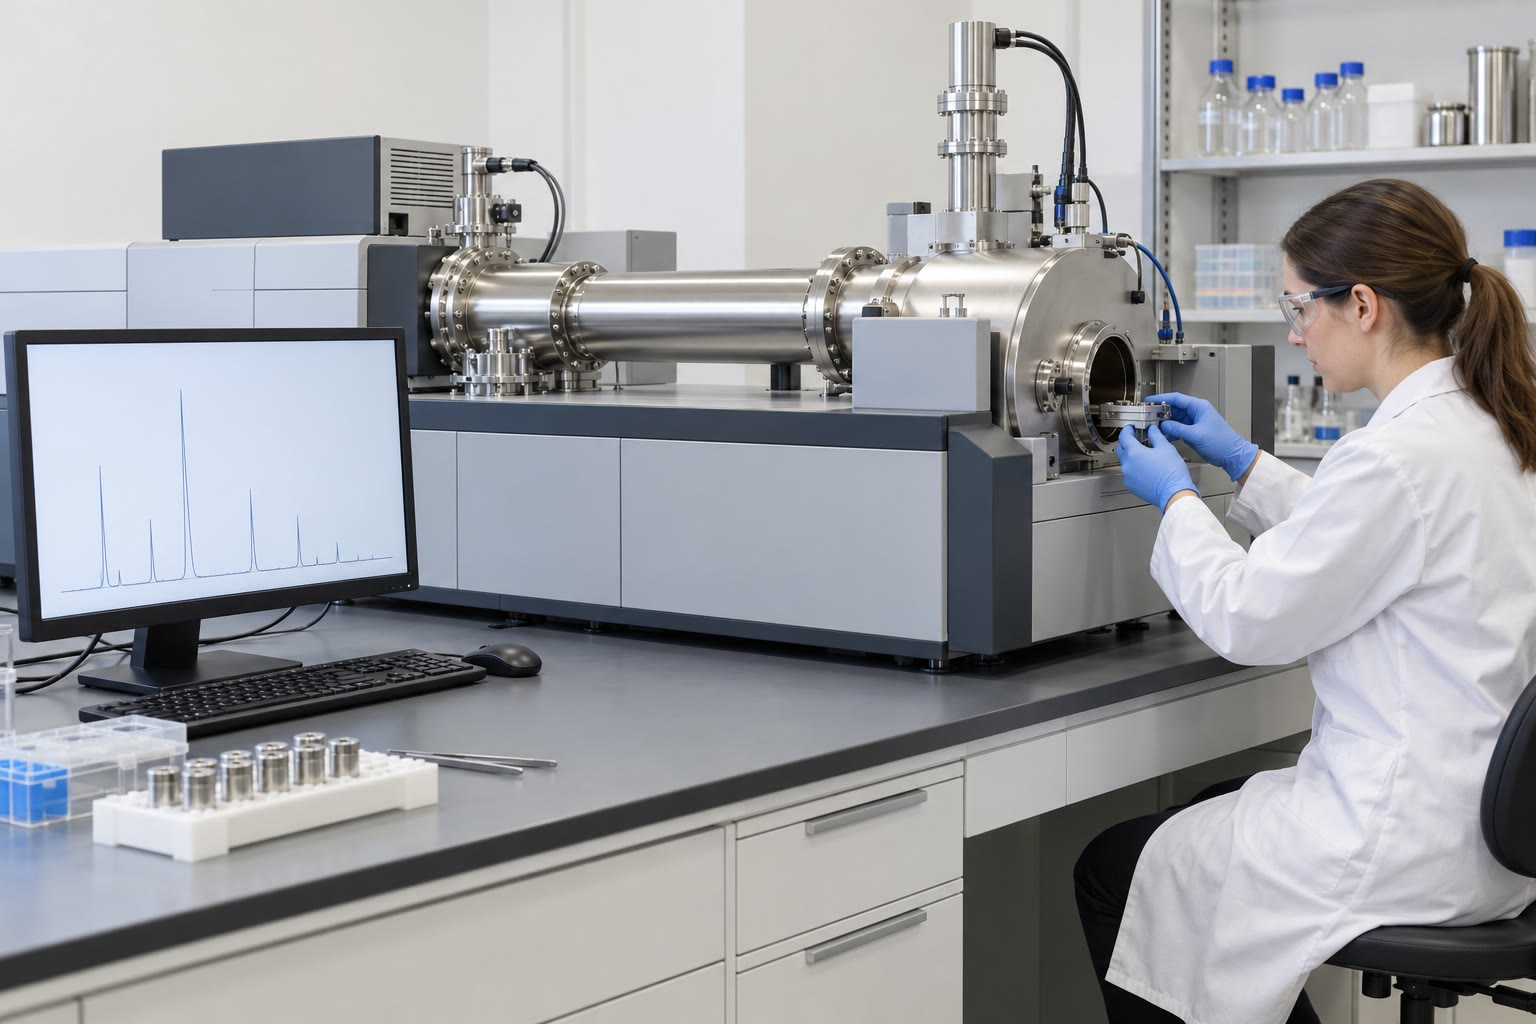
\includegraphics[width=0.66\linewidth]{images/book2/ai/g12-mass-spectrometer-lab.jpg}

{\small A mass spectrometer in a laboratory: a sample is being loaded at the
source end. AI-generated illustration.}
\end{omfigure}

The starting ratio is also a clue to where the magma came from. Rubidium
prefers the melt when the mantle melts, so over the ages it has been
concentrated in the \omterm{def:g12:continental-crust:continental-crust}{continental crust}, which has therefore made more
strontium-87: crustal rocks have a higher $^{87}\mathrm{Sr}/^{86}\mathrm{Sr}$
than mantle rocks. A magma from melted crust inherits that high ratio.
% ledger: tulane:radiometric

\section{The age of the Earth}

No rock on Earth goes back to the Earth's beginning: the oldest known rock,
the Acasta gneiss, is 4.03 billion years old, and the oldest zircons 4.4
billion. The surface has been melted, eroded and recycled since. The dating
of the Earth itself comes from meteorites, fragments of the small bodies
that formed with the planets and some of which have stayed \omterm{def:g12:age-of-the-earth:closed-system}{closed systems}
ever since.
% ledger: bowring99:acasta, wilde01:zircon, usgs:age-earth (Book 1 row)

\begin{definition}[Age of the Earth]\label{def:g12:age-of-the-earth:age}
The \emph{age of the Earth}\index{age of the Earth} is the time since the
Earth formed by the accretion of smaller bodies, at the birth of the Solar
System. Measured from meteorites by radiometric dating, it is
\num{4.54} billion years, to within one per cent.
\end{definition}
% ledger: usgs:age-earth (Book 1 row)

In 1956 Clair Patterson measured the isotopes of lead in three stony
meteorites and two iron meteorites. Two isotopes of lead are made by the
decay of uranium, lead-206 from uranium-238 and lead-207 from uranium-235,
while lead-204 is made by no decay. Like strontium, the points of meteorites
that formed at the same time lie on a straight line, when
$^{207}\mathrm{Pb}/^{204}\mathrm{Pb}$ is plotted against
$^{206}\mathrm{Pb}/^{204}\mathrm{Pb}$. The iron meteorite of Canyon Diablo, in
Arizona, holds almost no uranium: its lead has not changed since it formed,
and marks the bottom end of the line, the lead the Solar System started with.
% ledger: patterson56:table, patterson56:constants, usgs:age-earth (Book 1 row: Canyon Diablo troilite)

\begin{omfigure}
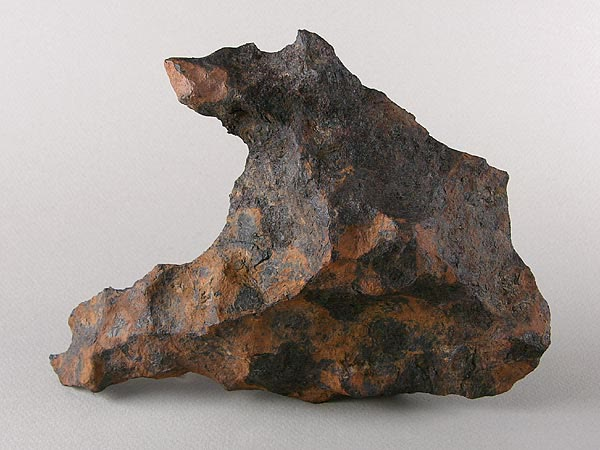
\includegraphics[height=4.2cm]{images/book2/g12-canyon-diablo-meteorite.jpg}

{\small A fragment of the Canyon Diablo iron meteorite, \qty{2641}{g}.
Photograph Geoffrey Notkin, CC~BY-SA~2.5 (Wikimedia Commons).}
\end{omfigure}
% ledger: photo:g12-canyon-diablo

For lead the slope $m$ depends on the age through both uranium isotopes; the
relation is admitted here. With the constants Patterson used,
\[
  m = \frac{1}{137.8}\,\frac{e^{\lambda_{235}t}-1}{e^{\lambda_{238}t}-1},
  \qquad \lambda_{235} = \num{9.72e-10},\ \lambda_{238} = \num{1.537e-10}
  \text{ per year},
\]
which gives:
\begin{center}
\small
\begin{tabular}{|l|c|c|c|c|c|c|}
\hline
age (billion years) & 4.40 & 4.45 & 4.50 & 4.55 & 4.60 & 4.65 \\
slope $m$ & 0.533 & 0.551 & 0.570 & 0.590 & 0.610 & 0.632 \\
\hline
\end{tabular}
\end{center}
% ledger: patterson56:constants
% values: pb_slope at 4.40-4.65 Ga (isochrons.py pb_slope)

\begin{omfigure}
\begin{tikzpicture}
\begin{axis}[omrecord, width=0.72\linewidth, height=6cm, xmin=0, xmax=56, ymin=0, ymax=40,
  xlabel={$^{206}\mathrm{Pb}/^{204}\mathrm{Pb}$}, ylabel={$^{207}\mathrm{Pb}/^{204}\mathrm{Pb}$}]
% computed in figdata/grade-12/isochrons.py; ledger: patterson56:table
\addplot[omDef, line width=0.9pt] table[x=x, y=y] {figdata/out/grade-12-isochrons-pbln.dat};
\addplot[omThm, only marks, mark=*, mark size=2pt] table[x=r206, y=r207, restrict expr to domain={\thisrow{idx}}{1:5}] {figdata/out/grade-12-isochrons-pbpb.dat};
\addplot[black, only marks, mark=o, mark size=2.6pt, line width=0.8pt] table[x=r206, y=r207, restrict expr to domain={\thisrow{idx}}{6:6}] {figdata/out/grade-12-isochrons-pbpb.dat};
\coordinate (nl) at (axis cs:50.28,34.86);
\coordinate (fc) at (axis cs:19.48,15.76);
\coordinate (cd) at (axis cs:9.5,10.36);
\coordinate (sed) at (axis cs:19.0,15.5);
\coordinate (sl) at (axis cs:30,25);
\end{axis}
\node[font=\scriptsize, anchor=north west] at ([xshift=2pt]nl) {Nuevo Laredo};
\node[font=\scriptsize, anchor=north west, align=left] at ([xshift=4pt, yshift=-2pt]fc) {Forest City, Modoc;\\ocean sediment (circle)};
\node[font=\scriptsize, anchor=north west, align=left] at ([xshift=3pt, yshift=-3pt]cd) {Canyon Diablo, Henbury (iron)};
\node[font=\scriptsize, text=omDef, anchor=south east] at (sl) {slope 0.603: about 4.6 billion years};
\end{tikzpicture}

{\small Patterson's lead \omterm{def:g12:age-of-the-earth:isochron}{isochron}: the five meteorites lie on one line, and
so, nearly, does lead from a modern ocean sediment, standing for the Earth.
Source: Patterson (1956), Table~1.}
\end{omfigure}
% values: pb_slope 0.6026, pb_age_Ga 4.58, sediment_residual -0.39 (isochrons.py)

A line drawn through the five points has a slope of about 0.603, between
the slopes for 4.55 and 4.60 billion years on the table. Patterson's own
result, allowing for the errors of the measurements and of the decay
constants, was 4.55 billion years, give or take 0.07. He then measured lead from a modern ocean sediment, which mixes
lead from a great mass of the Earth's crust: it lies on the same line. The
Earth's lead has evolved like that of the meteorites, over the same time: the
Earth is as old as they are.
% ledger: patterson56:table

Since then, hundreds of measurements have confirmed it. Meteorites give ages
from 4.53 to 4.58 billion years, and the oldest solids of the Solar System,
small inclusions rich in calcium and aluminium found in some meteorites,
formed \num{4567.30} million years ago, give or take 0.16. The Earth formed
later from such material, which is why its age, 4.54 billion years, is a
little less than theirs.
% ledger: usgs:age-earth (Book 1 row), connelly12:cai

\section{Exercises}

\begin{exercise}[$\star$]\label{exo:g12:age-of-the-earth:1}
Give the word: (a) a mineral into and out of which no parent or daughter atom
has moved since its clock started; (b) the straight line on which minerals of
one age and one source plot; (c) the time since the Earth formed by
accretion.
\end{exercise}

\begin{exercise}[$\star$]\label{exo:g12:age-of-the-earth:2}
Using the table of the Varden granite, put its five samples in the order of
their ratio of rubidium-87 to strontium-86, from the lowest. Which of them
plots highest on the \omterm{def:g12:age-of-the-earth:isochron}{isochron}, and why has it made the most strontium-87?
\end{exercise}

\begin{exercise}[$\star$]\label{exo:g12:age-of-the-earth:3}
Compute the half-life of rubidium-87 from its decay constant,
\num{1.3972e-11} per year. How many times the \omterm{def:g12:age-of-the-earth:age}{age of the Earth} is it?
\end{exercise}

\begin{exercise}[$\star$]\label{exo:g12:age-of-the-earth:4}
Compute $e^{\lambda t} - 1$ for rubidium-87 for $t = 310$ million years and
$t = 480$ million years.
\end{exercise}

\begin{exercise}[$\star$]\label{exo:g12:age-of-the-earth:5}
Put in order of date the estimates of Phillips, Holmes (1927), Joly, Kelvin
(1862) and Patterson. How many times larger than the upper end of Joly's
estimate is today's \omterm{def:g12:age-of-the-earth:age}{age of the Earth}?
\end{exercise}

\begin{exercise}[$\star\star$]\label{exo:g12:age-of-the-earth:6}
A mineral of the Varden granite (310 million years, starting ratio 0.7080)
has $^{87}\mathrm{Rb}/^{86}\mathrm{Sr} = 10.0$. What is its
$^{87}\mathrm{Sr}/^{86}\mathrm{Sr}$ today? What was it when the granite
formed?
\end{exercise}

\begin{exercise}[$\star\star$]\label{exo:g12:age-of-the-earth:7}
Four samples of the Varden schist give $(x, y)$ = (0.90, 0.71806),
(2.60, 0.72950), (5.10, 0.74632) and (9.40, 0.77525), with $x =
{}^{87}\mathrm{Rb}/^{86}\mathrm{Sr}$ and $y = {}^{87}\mathrm{Sr}/^{86}\mathrm{Sr}$.
(1) From the first and last samples, compute the slope and the age.
(2) Check that the two middle samples lie on the same line. (3) Is the
result consistent with the granite's 310 million years and the principle of
cross-cutting relationships?
\end{exercise}

\begin{exercise}[$\star\star$]\label{exo:g12:age-of-the-earth:8}
Why does a rock in which all the minerals have the same ratio of rubidium to
strontium give no \omterm{def:g12:age-of-the-earth:isochron}{isochron}? Why does the biotite, in the Varden granite,
fix the slope better than the other minerals?
\end{exercise}

\begin{exercise}[$\star\star$]\label{exo:g12:age-of-the-earth:9}
Long after the Varden granite formed, a hot fluid made its biotite lose part
of its strontium-87. (1) Where does its point move on the \omterm{def:g12:age-of-the-earth:isochron}{isochron} diagram?
(2) What age would the biotite and the plagioclase alone then give: too old or
too young? (3) How does the \omterm{def:g12:age-of-the-earth:isochron}{isochron} method reveal the problem?
\end{exercise}

\begin{exercise}[$\star\star$]\label{exo:g12:age-of-the-earth:10}
(1) How many times longer than Kelvin's 96 million years is the \omterm{def:g12:age-of-the-earth:age}{age of the
Earth}? (2) Joly assumed that the rivers bring salt to the sea at a steady
rate and that none of it leaves the sea. Which of these assumptions makes his
age too short if it is wrong, and why?
\end{exercise}

\begin{exercise}[$\star\star$]\label{exo:g12:age-of-the-earth:11}
Using Patterson's values for Canyon Diablo (9.46, 10.34) and Nuevo Laredo
(50.28, 34.86), compute the slope of the line through the two meteorites,
and read the age from the table of slopes.
\end{exercise}

\begin{exercise}[$\star\star\star$]\label{exo:g12:age-of-the-earth:12}
A basalt of the Varden region, also 310 million years old, has a starting
ratio of 0.7035, against 0.7080 for the granite. (1) Which rock is more
likely to come from melted mantle, and which from melted crust? (2) Explain
why with what you know of rubidium. (3) Could the two have crystallised from
one magma?
\end{exercise}

\begin{exercise}[$\star\star\star$]\label{exo:g12:age-of-the-earth:13}
(1) What fraction of the rubidium-87 present when the Earth formed is left
today? And of the uranium-238 (half-life 4.47 billion years)? (2) What would
be the slope of a rubidium--strontium \omterm{def:g12:age-of-the-earth:isochron}{isochron} for a rock one million years
old? Why is rubidium--strontium a poor clock for young rocks?
\end{exercise}

\begin{exercise}[$\star\star\star$]\label{exo:g12:age-of-the-earth:14}
The line through Patterson's five meteorites is $y = 4.438 + 0.6026\,x$.
(1) What $^{207}\mathrm{Pb}/^{204}\mathrm{Pb}$ does it predict for the ocean
sediment, at $x = 19.0$? Patterson measured 15.5: by what percentage do they
differ? (2) What age does the slope 0.6026 give, from the table? Compare with
Patterson's $4.55 \pm 0.07$ billion years.
\end{exercise}

\begin{exercise}[$\star\star\star$]\label{exo:g12:age-of-the-earth:15}
Kelvin supposed that all the heat the Earth loses, \qty{46.7}{TW} today, is
stored heat. (1) Radioactivity replaces about \qty{24.4}{TW} of it. By how
much does that, alone, lengthen the time to lose a given store of heat?
(2) Starting from 96 million years, is this enough to reach the true age?
(3) What did Kelvin miss that matters more?
\end{exercise}

\begin{problem}[{Weekend problem --- Dating the Varden granite}]
\label{pb:g12:age-of-the-earth:1}
% exercise data from figdata/grade-12/isochrons.py; ledger: villa22:rb87, tulane:radiometric, ics:base.Carboniferous, ics:base.Permian
The granite of the Varden Hills, the series' invented region, cuts the
schist around it. A laboratory measured five of its samples (example above):
plagioclase (0.35, 0.70952), hornblende (1.20, 0.71321), whole rock (3.10,
0.72146), K-feldspar (6.40, 0.73578) and biotite (24.0, 0.81218), each as
$(^{87}\mathrm{Rb}/^{86}\mathrm{Sr},\ ^{87}\mathrm{Sr}/^{86}\mathrm{Sr})$. The
decay constant of rubidium-87 is \num{1.3972e-11} per year.

\medskip
\noindent\textbf{Part I --- The samples.}
\begin{enumerate}
  \item Which sample is the richest in rubidium relative to strontium?
  \item Why did all the minerals start with the same
        $^{87}\mathrm{Sr}/^{86}\mathrm{Sr}$?
  \item Why are the ratios taken to strontium-86?
  \item Which of the three isotopes has grown since the granite formed, and
        why?
  \item What did the five points look like on the diagram when the granite
        had just formed?
\end{enumerate}

\medskip
\noindent\textbf{Part II --- The isochron line.}
\begin{enumerate}[resume]
  \item Compute the slope through the plagioclase and the biotite.
  \item Compute the slope through the plagioclase and the whole rock.
  \item Compare the two slopes. Which is the more reliable, and why?
  \item Find where the line of question 6 meets the vertical axis.
  \item Check that the K-feldspar lies on that line.
\end{enumerate}

\medskip
\noindent\textbf{Part III --- The slope and the age.}
\begin{enumerate}[resume]
  \item Write the relation between the slope and $e^{\lambda t}$.
  \item Compute $\lambda t$.
  \item Compute the age $t$.
  \item The schist has been dated at 480 million years. Is the order of the
        two ages what the field relations require?
  \item The Carboniferous runs from 358.9 to 298.9 million years ago. In
        which period did the granite form?
\end{enumerate}

\medskip
\noindent\textbf{Part IV --- The starting ratio and the source.}
\begin{enumerate}[resume]
  \item What does the intercept, 0.7080, represent?
  \item A basalt of the region formed with a ratio of 0.7035. Which rock
        has the higher starting ratio?
  \item Why do crustal rocks have higher ratios than the mantle?
  \item What does the granite's starting ratio suggest about the rock that
        melted to make it?
  \item Sum up: how old is the Varden granite?
\end{enumerate}
\end{problem}
